%!TEX root = TQFTnotes.tex
%%%%%%%%%%%%%%%%%%%%%%%%%%%%%%
\chapter{Category of cobordisms and definition of TQFT}\label{c:cobordisms}

In this chapter, we give the key definition of this book, namely the notion of a
TQFT, following work of Atiyah (see \cite{atiyah}). To do that, we first define
the notion of a cobordism.

Unless specified otherwise, ``manifold'' means a compact oriented smooth
manifold, possibly with boundary. For a manifold $M$, we denote by $\del M$ its
boundary, with the orientation determined by the orientation of $M$. If $\del
M=\varnothing$, we say that $M$ is \emph{closed}. Morphisms between manifolds
are smooth maps; unless stated otherwise, ``diffeomorphism'' means an
orientation-preserving invertible smooth map.

We denote by $\ov{M}$ the manifold $M$ considered with the
opposite orientation.

The main references for this chapter are \cite{kock} and
\cite{milnor-h-cobordism}.

%%%%%%%%%%%%%%%%%%%
\section{Category $\nCob$ and definition of TQFT}\label{s:TQFT-def}
\begin{definition}\label{d:cobordism}\index{cobordism}
Let $N_0, N_1$ be closed $(n-1)$-dimensional manifolds. A \emph{cobordism}
from $N_0$ to $N_1$ is an $n$-dimensional manifold $M$ together with
an isomorphism
$$
  \ph\colon \ov{N_0}\sqcup N_1 \isoto \del M.
$$
We will refer to $N_0$ as the incoming boundary (or simply the in-boundary),
and to $N_1$ as the outgoing boundary (out-boundary).

Following \cite{kock}, we will write $N_0\cob{M} N_1$ to indicate that $M$ is a
cobordism from $N_0$ to $N_1$.
\end{definition}

The picture below shows a 2-dimensional cobordism between a circle and a union
of two circles; this cobordism is usually called \emph{pair of pants}\index{pair of pants}.
\begin{center}
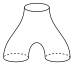
\includegraphics{figures/c3-fig01.svg}
\end{center}

\begin{convention}
In our pictures, cobordisms go ``top to bottom'':
the in-boundary is at the top, and the out-boundary is at the bottom.
\end{convention}

\begin{definition}\label{d:cobordism-isomorphism}\index{cobordism!isomorphism}
  An isomorphism of two cobordisms $M_1, M_2\in \nCob(N_0,N_1)$ is a
  diffeomorphism $f\colon M_1\to M_2$ which makes this diagram commutative:
  \begin{equation}\label{e:cob-iso}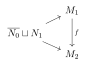
\includegraphics{figures/c3-fig02.svg}\end{equation}
\end{definition}
Given two cobordisms $N_0\cob{M_1}N_1$, $N_1\cob{M_2}N_2$, it is natural to
ask if they can be glued together in a single cobordism $M=M_2\circ M_1$
$$
  N_0\cob{M_2\circ M_1}N_2.
$$
Clearly, as a manifold, $M$ should be obtained by gluing $M_1$ and $M_2$ along
the common boundary $N_1$: $M= M_1\cup_{N_1} M_2$. However, there is a problem:
it is easy to define $M$ as a topological space, but the smooth structure is not
unique. There are several ways to deal with this problem.
\begin{itemize}
  \item One can switch to the category of PL manifolds and cobordisms,
    where the problem does not arise: the PL structure on $M_1\cup_{N_1} M_2$
    is uniquely determined by the PL structures on $M_1$, $M_2$.
  \item One can consider \emph{collared}\index{collared manifold}
    manifolds: instead of
    isomorphism $\ov{N_0}\sqcup N_1\to \del M$,
    we can require in the definition of cobordism an isomorphism of
    $(\ov{N_0}\sqcup N_1)\times [0, \epsilon)$ with a neighborhood
    of $\del M$ in $M$.
\end{itemize}
However, the simplest way is to note that while the smooth structure is not
unique, different smooth structures give isomorphic cobordisms.

\begin{theorem}\label{t:gluing-unique}
  The smooth structure on $M=M_1\cup_{N_1} M_2$ which agrees with
  the given smooth structures on $M_1$, $M_2$, is unique up to isomorphism:
  if $\al, \al'$ are two different smooth structures on $M$, then $(M,\al)$,
  $(M,\al')$ are isomorphic as cobordisms.
\end{theorem}
You can find a proof of this in \cite[Theorem 1.3.12]{kock}.

\begin{definition}\label{d:ncob}\index{cobordism category}
  The cobordism category $\nCob$ is the category whose objects are closed
  $(n-1)$-dimensional manifolds, and $\Hom(N_0, N_1)$ is the set of
  isomorphism classes of cobordisms $N_0\cob{M}N_1$. The composition of
  cobordisms $N_0\cob{M_1}N_1$, $N_1\cob{M_2}N_2$
  is given by
  $$
    M_2\circ M_1 = M_1\cup_{N_1} M_2
  $$
  (by the previous theorem it is independent of the choice of smooth structure).
  The identity morphism $\id_N$ is the cylinder $N\times I$.
\end{definition}
Similarly one defines the PL version of cobordism category.

This category has a natural structure of a symmetric monoidal
category with respect to disjoint union.

\begin{definition}\label{d:tqft}\index{TQFT}
  An $n$-dimensional TQFT is a symmetric
  monoidal functor $Z\colon \nCob\to \vect$.
\end{definition}
This definition was first given in \cite{atiyah} in slightly different
language.

One can also generalize this definition, allowing the TQFT to take values in
other categories.

\begin{definition}\label{d:tqft-c}
  Let $\calC$ be a symmetric monoidal category. Then an
  $n$-dimensional TQFT with values in $\calC$ is a symmetric
    monoidal functor $Z\colon \nCob\to \calC$.
\end{definition}
%%%%%%%%%%%%%%%%%%%%%%%%%%%%
\section{1D TQFT}\label{s:1d-tqft}

Now that we have a definition of a TQFT, let us try to construct examples. We
begin with the simplest possible case, that of a 1-dimensional TQFT.

\begin{theorem}\label{t:1d-TQFT}
  A 1-dimensional TQFT is the following collection of data:
  \begin{itemize}
    \item A vector space $V_+=Z(\bullet^+)$
    \item A vector space $V_-=Z(\bullet^-)$
    \item A linear map $\ev= Z(\cup)\colon V_+\otimes V_-\to \kk$
    \item A linear map $\coev = Z(\cap)\colon \kk \to V_-\otimes V_+$
  \end{itemize}
  satisfying relations below.
  \begin{equation}\label{e:1d-tqft-rigidity}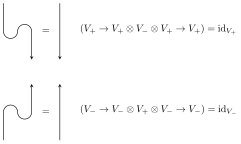
\includegraphics{figures/c3-eqfig01.svg}\end{equation}
\end{theorem}
\begin{proof}
  Since $Z$ is symmetric monoidal, $Z(N_1\sqcup N_2)\simeq Z(N_1)\otimes Z(N_2)$,
  so $Z$ on objects is determined by its values on connected 0-manifolds. The
  only connected 0-manifolds are the positively and negatively oriented points
  $\bullet^+, \bullet^-$, hence $Z$ on objects is determined by
  $V_\pm := Z(\bullet^\pm)$.

  Similarly, $Z$ on morphisms is determined by its values on connected
  cobordisms. Up to isomorphism, every connected oriented $1$-cobordism with
  non-empty boundary is one of the following:
  \begin{itemize}
    \item the intervals $\bullet^+\to\bullet^+$ and $\bullet^-\to\bullet^-$,
      on which $Z$ is the identity of $V_+$ resp.\ $V_-$;
    \item the \emph{cup}
      $\bullet^+\sqcup\bullet^-\to\varnothing$, on which $Z$ is a linear
      map $\ev\colon V_+\otimes V_-\to\kk$;
    \item the \emph{cap}
      $\varnothing\to\bullet^-\sqcup\bullet^+$, on which $Z$ is a linear
      map $\coev\colon \kk\to V_-\otimes V_+$.
  \end{itemize}
  The only connected closed $1$-cobordism is the circle $S^1$; its value
  $Z(S^1)\in\kk$ will turn out to be determined by the data above.

  It remains to identify the relations these data must satisfy. The snake
  cobordism on the left-hand side of the first equation of
  \eqref{e:1d-tqft-rigidity} is diffeomorphic (rel boundary) to the straight
  interval on the right-hand side; applying $Z$ to this diffeomorphism gives
  the first snake identity. The second is obtained analogously by reversing
  orientations.

  Conversely, given data $(V_+, V_-, \ev, \coev)$ satisfying
  \eqref{e:1d-tqft-rigidity}, one defines $Z$ on objects and connected
  cobordisms by the formulas above and extends to general objects and
  morphisms by tensor product and composition. The relations
  \eqref{e:1d-tqft-rigidity} ensure that the result is independent of the
  decomposition; with this, $Z$ is well-defined as a symmetric monoidal
  functor $\oneCob\to\vect$.
\end{proof}

\begin{lemma}\label{l:rigidity_vect}
  Let $V_+, V_-$, $\ev, \coev$ be as in \thref{t:1d-TQFT}.
  Then $V_+, V_-$ are finite-dimensional, and
  one can identify $V_-=V_+^*$ so that $\ev, \coev$ become the usual
  evaluation and coevaluation maps $V\otimes V^*\to \kk$,
  $\kk\to V\otimes V^*\colon 1\mapsto \sum e_i\otimes e^i$.
\end{lemma}
\begin{proof}
  Consider the map $V_-\to (V_+)^*$, given by $y\mapsto \ev(-,y)$; and a map
  $V_+^*\to V_-$ given by
  $f\mapsto \id \otimes f (\coev(1))$ (thus, if $\coev(1)=\sum y_i \otimes x_i$,
  then $f\mapsto \sum f(x_i) y_i$). Then the rigidity conditions say that these
  two maps are inverse to each other; thus, we have $V_-\simeq V_+^*$.
  Finite-dimensionality follows from the fact that the elements $y_i$ generate
  $V_-$.
\end{proof}
Thus, a one-dimensional TQFT is completely determined by a
\emph{finite-dimensional} vector space $V=Z(\bullet^+)$; in such a
TQFT, $Z(S^1)=\dim V$.


%%%%%%%%%%%%%%%%%%%%%%%%%
\section{Rigid monoidal categories}\label{s:1d-tqft-rigid}
In the previous section, we had shown that a 1d TQFT with values in the category
of vector spaces is uniquely determined by the vector space $V=Z(\bullet^+)$,
which must be finite-dimensional. What happens if we now consider TQFTs with
values in an arbitrary monoidal category $\calC$?

It turns out that there is a very similar answer, but with finite-dimensionality
replaced by the following condition.

\begin{definition}\label{d:dual-object}
  Let $\calC$ be a monoidal category.
  A \emph{dual pair}\index{dual pair} is a pair of objects $A,B\in \calC$
  together with morphisms
  \begin{align*}
    \ev&\colon A\otimes B\to \one \qquad \text{(evaluation morphism),}\\
    \coev&\colon \one \to B\otimes A \qquad \text{(coevaluation morphism)},
  \end{align*}
  satisfying the \emph{rigidity}\index{rigidity} condition below.
  \begin{equation}\label{e:rigidity}
    \begin{aligned}
      &\Bigl(B\to \one\otimes B \xto{\coev\otimes 1_B}
                       (B\otimes A)\otimes B \xto{\al_{B,A,B}}
                       B\otimes (A\otimes B) \xto{1_B\otimes \ev}
                       B\otimes \one \to
                       B\Bigr) = 1_B\\
      &\Bigl(A\to  A\otimes \one  \xto{1_A\otimes \coev}
                       A\otimes (B\otimes A) \xto{\al^{-1}_{A,B,A}}
                       (A\otimes B)\otimes A \xto{\ev\otimes 1_A}
                       \one\otimes A \to
                       A\Bigr) = 1_A
    \end{aligned}
  \end{equation}
  In this situation we say that $A$ is a
  \emph{left dual}\index{dual object!left} of $B$, and
  $B$ is a \emph{right dual}\index{dual object!right} of $A$.
\end{definition}

It is common to represent the evaluation and coevaluation graphically:
\begin{equation}\label{e:ev-coev-graphical}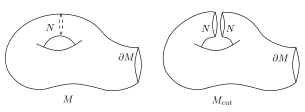
\includegraphics{figures/c3-fig03.svg}\end{equation}

Then the rigidity equations \eqref{e:rigidity} are illustrated by
\begin{equation}\label{e:rigidity2}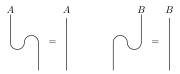
\includegraphics{figures/c3-eqfig02.svg}\end{equation}



It turns out that right dual, if exists, is unique up to unique isomorphism.
\begin{theorem}\label{t:dual_unique1}
  Let $(A, B, \ev, \coev)$ and $(A,B', \ev', \coev')$ be two dual pairs with
  the same $A$.
  Then there exists a unique morphism $\ph\colon B\to B'$ such that
  $\ev = \ev' \circ (1_A\otimes \ph)$,
  $\coev' =(\ph\otimes 1_A) \coev$.
\end{theorem}
The proof is a standard snake-diagram argument: the required $\ph$ is given by
the composition
$$
  B \xto{1_B\otimes \coev'} B\otimes A\otimes B'
    \xto{\ev\otimes 1_{B'}} B',
$$
and uniqueness follows by chasing the rigidity equations.
A similar statement holds for left dual.

This allows us to talk about the right dual of $A$ as a well-defined object in
$\calC$. We will denote the right dual of $A$ by ${}^*A$; similarly we will use
notation $B^*$ for left dual of $B$. In this notation, evaluation and
coevaluation morphisms become
\begin{equation}
  \begin{aligned}
    \ev&\colon X^*\otimes X\to\one\\
    \coev&\colon \one \to X\otimes X^*.
  \end{aligned}
\end{equation}

Clearly, in a symmetric monoidal
category, the left dual is also a right dual.

\begin{definition}\label{d:rigid}
  An object $A$ in a monoidal category $\calC$ is
  \emph{rigid}\index{rigid object} if
  it has both left and right duals.

  A monoidal category is \emph{rigid}\index{monoidal category!rigid}
  if every object is rigid.
\end{definition}

\begin{example}\label{x:vector-rigid}
  A vector space $V$ is rigid as an object of $\vect$ if and only if it is
  finite-dimensional.
\end{example}


\begin{exercise}\label{ec:coev-unique}
  Show that in a dual pair, the coevaluation is uniquely determined by
  the remaining data: if $(A, B, \ev, \coev)$ and $(A,B, \ev, \coev')$
  are dual pairs, then $\coev = \coev'$.

  Similarly, $\ev$ is uniquely determined by $(A,B, \coev)$.
\end{exercise}

\begin{exercise}\label{ec:dual-of-tensor}
  Let $X^*$, $Y^*$ be right duals of objects $X, Y$. Show that then $X\otimes Y$
  also has a right dual, and there is a canonical isomorphism $(X\otimes
  Y)^*\simeq Y^* \otimes X^*$.
\end{exercise}

\begin{exercise}\label{ec:dual-morphism}
  Let $\calC$ be a rigid monoidal category. For a morphism $f\colon X\to Y$,
  define a morphism $f^*\colon Y^*\to X^*$ by the picture below.

  \begin{equation}\label{e:dual-morphism}
\includegraphics{figures/c3-fig04.svg}\end{equation}


  Prove that then
  $(fg)^*=g^* f^*$; thus, $*$ is a contravariant functor $\calC\to \calC$.
\end{exercise}

After these preliminaries, we can now easily classify 1-dimensional TQFTs with
values in any symmetric monoidal category.

\begin{theorem}\label{t:1d-tqft}
  If $Z\colon \oneCob\to \calC$ is a $1$-dimensional TQFT with values in a
  symmetric monoidal category $\calC$, then $A=Z(\bullet^+)$ is a rigid object;
  its dual is $Z(\bullet^-)$. Conversely, any rigid object $A\in \calC$ defines
  a one-dimensional TQFT such that $Z(\bullet^+)=A$.
\end{theorem}

%\begin{tikzpicture}
%  \begin{scope}[tikzdefault]
%  \draw[->] (-0.5,0) arc (-180:0:0.5);
%  \draw[-] (0.5,0) arc (0:180:0.5);
%  \end{scope}
%\end{tikzpicture}


%%%%%%%%%%%%%%%%%%%%%
\section{First properties of TQFTs}\label{s:first-properties}



Let us now try to establish some properties of general $n$-dimensional TQFTs.

\begin{theorem}\label{t:tqft-rigidity}
  Let $Z\colon \nCob\to \calC$ be an $n$-dimensional TQFT with values in a
  symmetric monoidal category $\calC$. Then for any closed $(n-1)$-dimensional
  manifold $N$, $Z(N)\in \calC$ is rigid, and $Z(\ov{N})$ is a dual of $Z(N)$.
\end{theorem}
The proof is the same as in the one-dimensional case.

In particular, for TQFTs with values in $\vect$, for any closed
$(n-1)$-dimensional manifold $N$, the vector space $Z(N)$ is finite-dimensional.

\begin{exercise}\label{ec:tqft-duality}
  Let $Z$ be an $n$-dimensional TQFT with values in $\vect$. Prove that then
  $Z(N\times S^1)=\dim Z(N)$ for any closed $(n-1)$-dimensional manifold $N$.
\end{exercise}

Note that unlike the one-dimensional case, in general we cannot claim that any
rigid object of $\calC$ defines a TQFT. The proper generalization of that
statement is the cobordism hypothesis, which we will discuss later.



Another property of TQFTs is functoriality. As mentioned before, it is
natural to expect that a diffeomorphism $\ph \colon N_0\to N_1$ between two
$(n-1)$-dimensional closed manifolds gives rise to an isomorphism
$Z(\ph)\colon Z(N_0)\to Z(N_1)$; however, we didn't include that as part of
the definition. It turns out it is not necessary.

Let $\ph \colon N_0\to N_1$ be a diffeomorphism. Define the cobordism
\begin{equation}\label{e:Cph}
  N_0\cob{C_\ph} N_1
\end{equation}
to be the cylinder $N_1\times I$, with the identification $\ov{N_0}\sqcup N_1
\to \del C_\ph$ given by $\ph\sqcup \id$.

\begin{lemma}\label{l:tqft-isotopy}
  Let $C_\ph$ be defined above. Then:
  \begin{enumerate}
    \item The isomorphism class of $C_\ph$ \textup{(}as a cobordism\textup{)} only depends on the
    isotopy class of $\ph$: if $\ph, \ph'$ are isotopic to each other, then
      $C_\ph\simeq C_{\ph'}$.
    \item Given diffeomorphisms $\ph_1\colon N_0\to N_1$, $\ph_2\colon N_1\to
      N_2$, we have an isomorphism of cobordisms
      $$
        C_{\ph_2}\circ C_{\ph_1}\simeq C_{\ph_2 \ph_1}.
      $$
  \end{enumerate}
\end{lemma}
Recall that $\ph, \ph'$ are called isotopic if there exists a one-parameter
family $\ph_t$ of smooth maps $N_0\to N_1$ such that $\ph_t$ is a diffeomorphism
for all $t$, and $\ph_0=\ph$, $\ph_1=\ph'$.

We leave the proof of this lemma as an easy exercise to the reader.

\begin{remark}
  In fact, there is a stronger statement: $C_\ph\simeq C_{\ph'}$ if and only if
  $\ph, \ph'$ are \emph{pseudo-isotopic}\index{pseudo-isotopic}, see
  \cite[Theorem 1.9]{milnor-h-cobordism}.
\end{remark}




As an immediate corollary, we get the following theorem.
\begin{theorem}\label{t:tqft-functoriality}
  Let $Z\colon \nCob\to \calC$ be an $n$-dimensional TQFT.
  \begin{enumerate}
    \item For any diffeomorphism $\ph\colon N_0\to N_1$, define
      $Z(\ph)\colon Z(N_0)\to Z(N_1)$ by $Z(\ph)=Z(C_\ph)$. Then
      $Z(\ph_2\ph_1)= Z(\ph_2)\circ Z(\ph_1)$.
    \item If $\ph_0,\ph_1$ are isotopic, then $Z(\ph_0)=Z(\ph_1)$.
  \end{enumerate}
\end{theorem}
\clearpage
